\documentclass{article}

\usepackage{color}
\usepackage[margin=1in]{geometry}
\usepackage{graphicx}
\usepackage{hyperref}
\usepackage{listings}

\definecolor{gray}{rgb}{0.5, 0.5, 0.5}
\definecolor{darkgreen}{rgb}{0, 0.6, 0}

\begin{document}
    \raggedright
    Homework 3 \break
    Christopher Seagraves
% % % % % % % % % % % % % % % % % % % % % % % % % % % % % % % % % % % % % % % % 

    \section*{Problem 1}
        \begin{minipage}{\linewidth}
            \raggedright
            I'm sorry for being lazy, but hopefully doing 6 or so nodes is enough to prove I could have continued...
            \begin{center}
                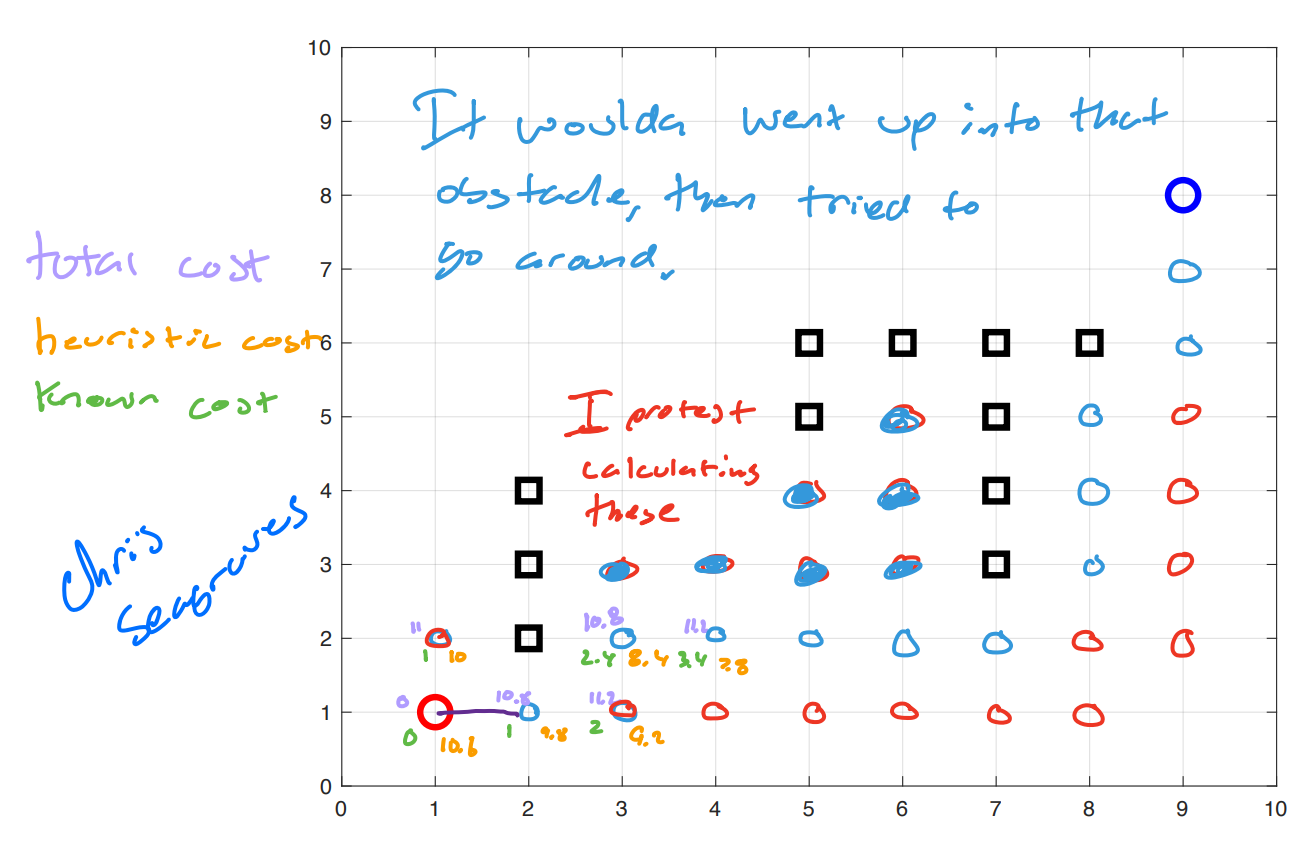
\includegraphics[width=\linewidth]{HW3P1 AStar by hand.png}
            \end{center}
        \end{minipage}
% % % % % % % % % % % % % % % % % % % % % % % % % % % % % % % % % % % % % % % %
    
        \section*{Problem 2}
            \begin{minipage}{\linewidth}
                \raggedright
                It should be noted, if you loop the obstacle list every iteration, this will take a long time. The solution is to put invalid nodes into a set and check if a given node exists in the set. \break 
                \break
                ./main.py \break
                \url{https://github.com/nosv1/seagraves_unmanned_systems/blob/main/SearchAlgorithms/main.py} \break
                ./AStar.py \break
                \url{https://github.com/nosv1/seagraves_unmanned_systems/blob/main/SearchAlgorithms/AStar.py}
                \begin{center}
                    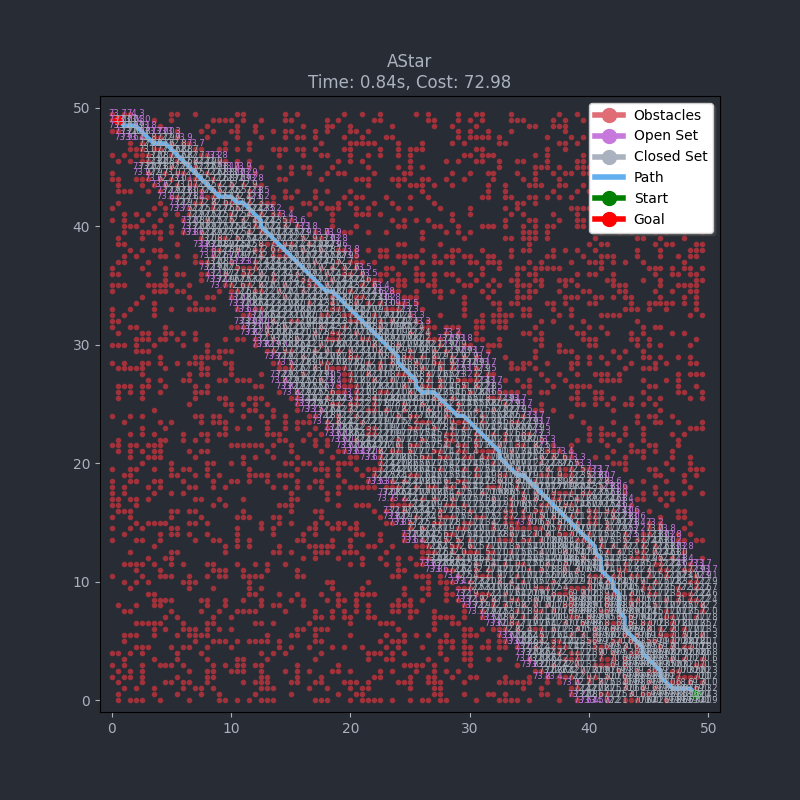
\includegraphics[width=\linewidth]{HW3P2 AStar.png}
                \end{center}
            \end{minipage}
% % % % % % % % % % % % % % % % % % % % % % % % % % % % % % % % % % % % % % % % 

        \section*{Problem 3}
            \begin{minipage}{\linewidth}
                \raggedright
                It should be noted, there does not exist a solution if you inflate the obstacles greater than the bot radius. For the plot, I didn't inflate the obstacles at all, so an obstacle is the size of one node. \break
                \break
                It should also be noted, the algorithim I used for stepping towards a node: \break
                \break
                - generate random node \break
                - step towards node from closest node \break
                - snap copy of node to grid \break
                - save stepped node if snapped node is a valid node \break
                \break
                This lets me use steps that aren't in the grid but still try and avoid obstacles. Like, for a more relaxed map - with more space between obstacles - I can inflate an obstacle, define the nodes in the obstacle as invalid, snap to a close node, check if it's invalid, and assume my 'non-snapped' node is valid or invalid.\break
                \break
                Something else you can do about these 'non-snapped' nodes, is when you take a step, you can take smaller steps along the line, and see if any of those steps are invalid - so you don't accidently step over a part of an obstacle. \break
                \break
                ./main.py \break
                \url{https://github.com/nosv1/seagraves_unmanned_systems/blob/main/SearchAlgorithms/main.py} \break
                ./RRT.py \break
                \url{https://github.com/nosv1/seagraves_unmanned_systems/blob/main/SearchAlgorithms/RRT.py}
                \begin{center}
                    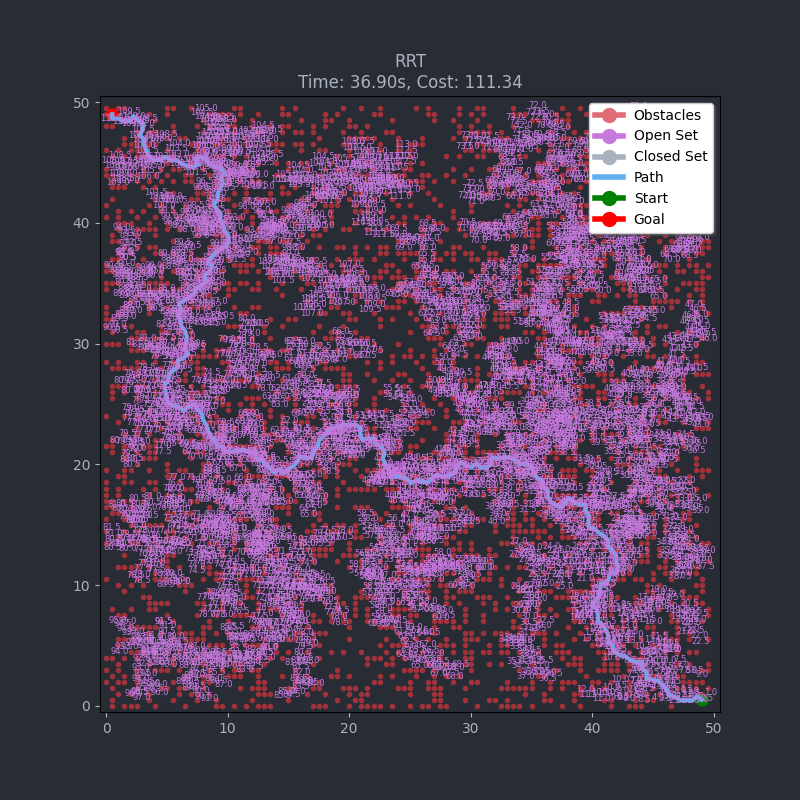
\includegraphics[width=\linewidth]{HW3P3 RRT.png}
                \end{center}
            \end{minipage}
% % % % % % % % % % % % % % % % % % % % % % % % % % % % % % % % % % % % % % % % 

\end{document}